\documentclass[a4paper,14pt]{extarticle}
\usepackage{../../tex-shared/preamble}

\renewcommand{\mylabnumber}{1}
\renewcommand{\mylabtitle}{Исследование возможностей языка разметки гипертекстов
                           HTML и каскадных таблиц стилей CSS}
\renewcommand{\mysubject}{Веб-технологии}
\renewcommand{\mylecturer}{Дрозин А.Ю.}

\begin{document}
\begin{titlepage}
    
    \thispagestyle{empty}
    
    \begin{center}
        
        Министерство науки и Высшего образования Российской Федерации \\
        Севастопольский государственный университет \\
        Кафедра ИС
        
        \vfill

        Отчет \\
        по лабораторной работе №\mylabnumber \\
        \enquote{\mylabtitle} \\
        по дисциплине \\
        \enquote{\MakeTextUppercase{\mysubject}}

    \end{center}

    \vspace{1cm}

    \noindent\hspace{7.5cm} Выполнил студент группы ИС/б-17-2-о \\
    \null\hspace{7.5cm} Горбенко К. Н. \\
    \null\hspace{7.5cm} Проверил \\
    \null\hspace{7.5cm} \mylecturer

    \vfill

    \begin{center}
        Севастополь \\
        2020
    \end{center}

\end{titlepage}
\lstset{ % "listings package configuration"
    basicstyle=\tiny\ttfamily,
}

\section{Цель работы}
Изучить основные понятия языка разметки гипертекстов HTML и
каскадных таблиц стилей CSS, исследовать структуру HTML-документа,
приобрести практические навыки реализации Web-страниц c
использованием гиперссылок, нумерованных и маркированных списков,
графических элементов, таблиц и форм ввода.

\section{Задание на работу}
В процессе выполнения лабораторной работы необходимо реализовать 
персональный Web-сайт. Рекомендуется наличие следующих веб-страниц
\begin{enumerate}
    \item Главная страница.
    \item Обо мне.
    \item Мои интересы.
    \item Учеба.
    \item Фотоальбом.
    \item Контакт.
    \item Тест по дисциплине.
\end{enumerate}

Задание для варианта №3. Тест по инженерной графике.
\begin{itemize}
    \item Radio2;
    \item Select4;
    \item Textarea.
\end{itemize}

\section{Ход работы}
\subsection{Результат}
Созданные HTML-страницы приведены в приложении.

Веб-страницы изображены на рисунках \ref{fig:homepage} - \ref{fig:test}.

\begin{figure}[H]
    \centering
    \includegraphics[width=.8\linewidth]{../images/homepage}
    \caption{Домашняя страница}
    \label{fig:homepage}
\end{figure}
\begin{figure}[H]
    \centering
    \includegraphics[width=.8\linewidth]{../images/about}
    \caption{Страница "Обо мне"}
    \label{fig:about}
\end{figure}
\begin{figure}[H]
    \centering
    \includegraphics[width=.8\linewidth]{../images/interests}
    \caption{Страница "Мои интересы"}
    \label{fig:interests}
\end{figure}
\begin{figure}[H]
    \centering
    \includegraphics[width=.8\linewidth]{../images/learning}
    \caption{Страница "Учеба"}
    \label{fig:learning}
\end{figure}
\begin{figure}[H]
    \centering
    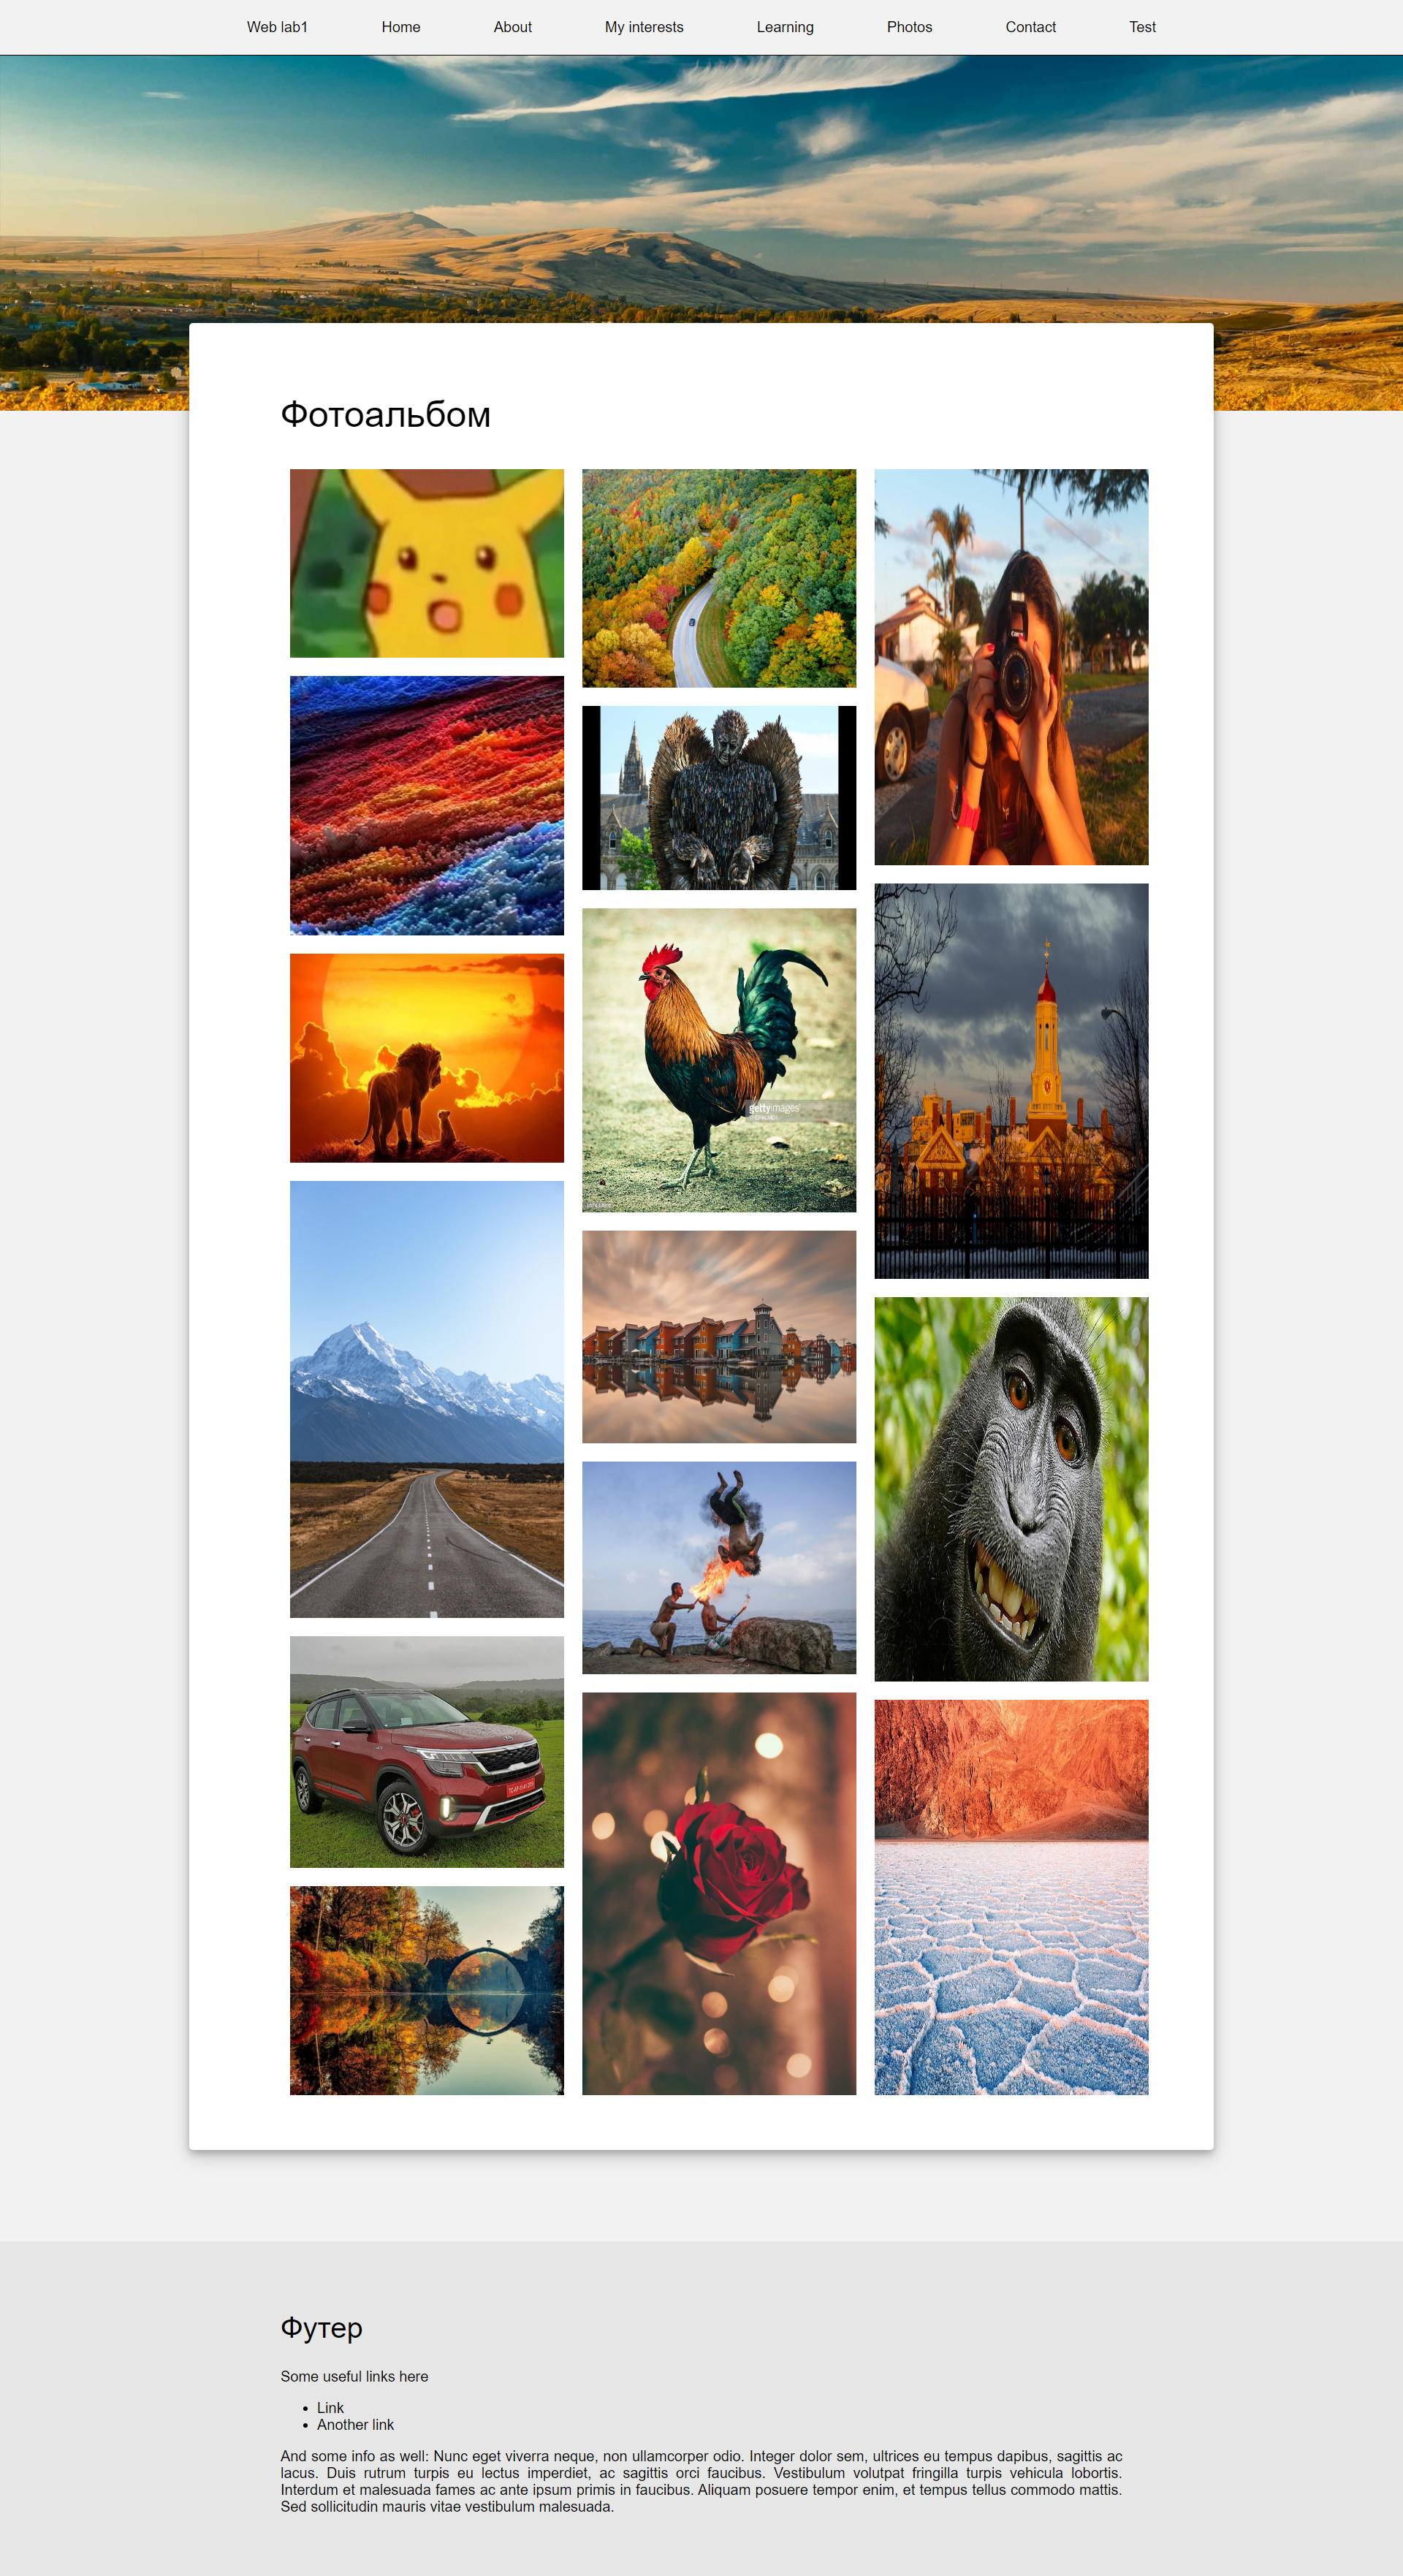
\includegraphics[width=.8\linewidth]{../images/photos}
    \caption{Фотоальбом}
    \label{fig:photos}
\end{figure}
\begin{figure}[H]
    \centering
    \includegraphics[width=.8\linewidth]{../images/contact}
    \caption{Страница "Контакт"}
    \label{fig:contact}
\end{figure}
\begin{figure}[H]
    \centering
    \includegraphics[width=.8\linewidth]{../images/test}
    \caption{Страница "Тест"}
    \label{fig:test}
\end{figure}

\subsection{Содержание страниц}
\subsubsection{Общее}
Все стриницы выполнены в одном стиле. Сверху находится
навигационная панель с названием сайта и ссылками на
все его страницы. Навигационная панель выполнена в
элементе \code{nav}, который является flex-контейнером.
Ссылки центрируются в зависимости от доступного места.
За навигационной панелью находится изображение, занимающее
всю ширину экрана.

Элемент, представляющий из себя содержание страницы, заступает
на картинку. Это выполнено при помощи свойства \code{top}.
Содержание выполнено при помощи элементов \code{section},
\code{p} и \code{h}.

Под содержанием находится футер. В нем можно расположить
некоторые ссылки или описания.

Общие стили задаются в файле \code{shared.css}.

\subsubsection{Главная страница}
На главной странице для фото задано свойство \code{float: left}
для обтекания ее текстом. При этом, чтобы контейнер, содержащий
картинку, не оказывался нулевой высоты, для него задано свойство
\code{overflow: hidden}.

\subsubsection{Страница \enquote{Обо мне}}
На странице присутствует нумерованный список и фотографии.

\subsubsection{Страница \enquote{Мои интересы}}
На странице в списке присутствуют ссылки с якорями для навигации.

\subsubsection{Страница \enquote{Учеба}}
На странице присутствует таблица. При этом шапка таблицы растянута
с помощью свойства \code{colspan}.

\subsubsection{Фотоальбом}
На странице расположен flex-контейнер, внутри которого фото
располагаются по столбцам.

\subsubsection{Странице \enquote{Контакт}}
На странице расположена форма для ввода данных пользователя.
Она содержит следующие элементы: \code{input type=text}, 
\code{input type=email}, \code{textfield} и кнопку подтверждения.

\subsubsection{Страница \enquote{Тест}}
На странице находится фома, состоящая из 2 элементов \code{radio},
элемента \code{select} с 3 опциями выбора и элемента \code{textfield}
для развернутого ответа. Кроме того, на странице находится стандартная
форма ввода данных пользователя со страницы "Контакт".

\section*{Выводы}
В ходе лабораторной работы был создан сайт-портфолио. Для этого
был применен язык разметки гипертекста HTML и каскадные таблицы
стилей CSS. Были применены семантические элементы HTML 5.

Для реализации некоторых элементов использовались flex-контейнеры,
но такое решение может не работать на более старых браузерах.
Кроме того, сайт не масштабируется для слишком узких экранов.
\section*{Приложение}
Главная страница:
\begin{lstlisting}
<!DOCTYPE html>

<html>
<head>
    <meta name="viewport" content="width=device-width" />
    <meta http-equiv="Cache-Control" content="no-cache, no-store, must-revalidate" />
    <link href="css/nav.css" rel="stylesheet" type="text/css" />
    <link href="css/shared.css" rel="stylesheet" type="text/css" />
    <link href="css/index.css" rel="stylesheet" type="text/css" />
    <title>Homepage</title>
</head>
<body>
    <nav>
        <ul class="nav-container">
            <li class="nav-item"><span                   >Web lab1</span></li>
            <li class="nav-item"><a href="index.html"    >Home</a></li>
            <li class="nav-item"><a href="about.html"    >About</a></li>
            <li class="nav-item"><a href="interests.html">My interests</a></li>
            <li class="nav-item"><a href="learning.html" >Learning</a></li>
            <li class="nav-item"><a href="photos.html"   >Photos</a></li>
            <li class="nav-item"><a href="contact.html"  >Contact</a></li>
            <li class="nav-item"><a href="test.html"     >Test</a></li>
        </ul>
    </nav>
    <img src="images/portrait.jpg" class="portrait">
    <div class="main-content">
        <header><h1>Портфолио</h1></header>
        <section>
            <img class="avatar" src="images/avatar.jpg" alt="author's avatar" title="that's me!">
            <header><h2>Обо мне</h2></header>
            <p>
                <i>Горбенко Кирилл Николаевич.</i> Группа ИС-17-2-о. Исследование возможностей
                языка разметки гипертекстов HTML и каскадных таблиц стилей CSS. 
                <strong>Вариант № 3</strong>.
            </p>

            <p>
                ...
            </p>
        </section>
        <section>
            <header><h2>Следующая глава</h2></header>

            <p>
                ...
            </p>
        </section>
    </div>
    <footer>
        <section>
            <header><h2>Футер</h2></header>
            <p>Some useful links here</p>
            <ul>
                <li>Link</li>
                <li>Another link</li>
            </ul>
            <p>
                ...
            </p>
        </section>
    </footer>
</body>
</html>
\end{lstlisting}

Страница "Обо мне"
\begin{lstlisting}
<!DOCTYPE html>

<html>
<head>
    <meta name="viewport" content="width=device-width" />
    <meta http-equiv="Cache-Control" content="no-cache, no-store, must-revalidate" />
    <link href="css/nav.css" rel="stylesheet" type="text/css" />
    <link href="css/shared.css" rel="stylesheet" type="text/css" />
    <link href="css/about.css" rel="stylesheet" type="text/css" />
    <title>About</title>
</head>
<body>
    <nav>
        <ul class="nav-container">
            <li class="nav-item"><span                   >Web lab1</span></li>
            <li class="nav-item"><a href="index.html"    >Home</a></li>
            <li class="nav-item"><a href="about.html"    >About</a></li>
            <li class="nav-item"><a href="interests.html">My interests</a></li>
            <li class="nav-item"><a href="learning.html" >Learning</a></li>
            <li class="nav-item"><a href="photos.html"   >Photos</a></li>
            <li class="nav-item"><a href="contact.html"  >Contact</a></li>
            <li class="nav-item"><a href="test.html"     >Test</a></li>
        </ul>
    </nav>
    <img src="images/portrait.jpg" class="portrait">
    <div class="main-content">
        <header><h1>Автобиография</h1></header>

        <section>
            <header><h1>Раздел 1</h1></header>

            <p>Здесь должна быть какая-то автобиография. Пускай тут будет списочек:</p>

            <ol>
                <li>19 лет.</li>
                <li>Сын своих родителей.</li>
                <li>Не знаю чего написать еще.</li>
                <li>Пойду заварю чайку.</li>
                <li>Заварил.</li>
                <li>Рыба меч дыня друг.</li>
            </ol>

            <p>Вот еще фоточки:</p>

            <div class="photo-wrapper">
                <img src="images/picachu.jpg" alt="funny picachu" title="Picachu!" />
                <img src="images/picachu.jpg" alt="funny picachu" title="Picachu!" />
                <img src="images/picachu.jpg" alt="funny picachu" title="Picachu!" />
                <img src="images/picachu.jpg" alt="funny picachu" title="Picachu!" />
                <img src="images/picachu.jpg" alt="funny picachu" title="Picachu!" />
                <img src="images/picachu.jpg" alt="funny picachu" title="Picachu!" />
            </div>
        </section>
    </div>
    <footer>
        <section>
            <header><h2>Футер</h2></header>
            <p>Some useful links here</p>
            <ul>
                <li>Link</li>
                <li>Another link</li>
            </ul>
            <p>
                ...
            </p>
        </section>
    </footer>
</body>
</html>
\end{lstlisting}

Страница "Мои интересы":
\begin{lstlisting}
<!DOCTYPE html>

<html>
<head>
    <meta name="viewport" content="width=device-width" />
    <meta http-equiv="Cache-Control" content="no-cache, no-store, must-revalidate" />
    <link href="css/nav.css" rel="stylesheet" type="text/css" />
    <link href="css/shared.css" rel="stylesheet" type="text/css" />
    <link href="css/interests.css" rel="stylesheet" type="text/css" />
    <title>Interests</title>
</head>
<body>
    <nav>
        <ul class="nav-container">
            <li class="nav-item"><span                   >Web lab1</span></li>
            <li class="nav-item"><a href="index.html"    >Home</a></li>
            <li class="nav-item"><a href="about.html"    >About</a></li>
            <li class="nav-item"><a href="interests.html">My interests</a></li>
            <li class="nav-item"><a href="learning.html" >Learning</a></li>
            <li class="nav-item"><a href="photos.html"   >Photos</a></li>
            <li class="nav-item"><a href="contact.html"  >Contact</a></li>
            <li class="nav-item"><a href="test.html"     >Test</a></li>
        </ul>
    </nav>
    <img src="images/portrait.jpg" class="portrait">
    <div class="main-content">
        <header><h1>Мои интересы</h1></header>
        <section>
            <header><h2>Contents</h1></header>
            <ul>
                <a class="contents" href="#hobby">Мое хобби.</a>
                <a class="contents" href="#books">Мои книги.</a>
                <a class="contents" href="#music">Моя музыка.</a>
                <a class="contents" href="#movies">Мои фильмы.</a>
            </ul>
        </section>
        <section id="hobby">
            <header><h2>Мое хобби:</h1></header>
            <p>Тут должны быть мои хобби</p>
            <p>
                ...
            </p>
            <p>
                ...
            </p>
        </section>

        <section id="books">
            <header><h1>Мои любимые книги:</h1></header>
            <p>Тут должны быть мои любимые книги</p>
            <p>
                ...
            </p>
            <p>
                ...
            </p>
        </section>

        <section id="music">
            <header><h1>Моя любимая музыка</h1></header>
            <p>Тут должны быть мои любимые исполнители</p>
            <p>
                ...
            </p>
            <p>
                ...
            </p>
        </section>

        <section id="movies">
            <header><h1>Мои любимые фильмы</h1></header>
            <p>Тут должны быть мои любимые фильмы</p>
            <p>
                ...
            </p>
            <p>
                ...
            </p>
        </section>
    </div>
    <footer>
        <section>
            <header><h2>Футер</h2></header>
            <p>Some useful links here</p>
            <ul>
                <li>Link</li>
                <li>Another link</li>
            </ul>
            <p>
                ...
            </p>
        </section>
    </footer>
</body>
</html>
\end{lstlisting}

Страница "Учеба":
\begin{lstlisting}
<!DOCTYPE html>

<html>
<head>
    <meta name="viewport" content="width=device-width" />
    <meta http-equiv="Cache-Control" content="no-cache, no-store, must-revalidate" />
    <link href="css/nav.css" rel="stylesheet" type="text/css" />
    <link href="css/shared.css" rel="stylesheet" type="text/css" />
    <link href="css/learning.css" rel="stylesheet" type="text/css" />
    <title>Learning</title>
</head>
<body>
    <nav>
        <ul class="nav-container">
            <li class="nav-item"><span                   >Web lab1</span></li>
            <li class="nav-item"><a href="index.html"    >Home</a></li>
            <li class="nav-item"><a href="about.html"    >About</a></li>
            <li class="nav-item"><a href="interests.html">My interests</a></li>
            <li class="nav-item"><a href="learning.html" >Learning</a></li>
            <li class="nav-item"><a href="photos.html"   >Photos</a></li>
            <li class="nav-item"><a href="contact.html"  >Contact</a></li>
            <li class="nav-item"><a href="test.html"     >Test</a></li>
        </ul>
    </nav>
    <img src="images/portrait.jpg" class="portrait">
    <div class="main-content">
        <section>
            <header><h1>Дисциплины</h1></header>
            <p>Институт информационных технологий и управления в технических системах</p>
            <p>Кафедра информационных систем</p>

            <table class="table">
                <tr class="table-row">
                    <td class="td" colspan="9">Дисциплины по семестрам</td>
                </tr>
                <tr class="table-row odd">
                    <th scope="row" class="th">1 семестр</td>
                    <td class="td">Высшая математика</td>
                    <td class="td">Алгоритмизация и программирование</td>
                    <td class="td">Информатика</td>
                    <td class="td">История</td>
                    <td class="td">Физика</td>
                    <td class="td">Экология</td>
                    <td class="td">Дискретная математика</td>
                    <td class="td">Английский язык</td>
                </tr>
                <tr class="table-row even">
                    <th scope="row" class="th">2 семестр</td>
                    <td class="td">Высшая математика</td>
                    <td class="td">Алгоритмизация и программирование</td>
                    <td class="td">Физика</td>
                    <td class="td">Философия</td>
                    <td class="td">Основы теории права</td>
                    <td class="td">Экономика</td>
                    <td class="td">БЖД</td>
                    <td class="td">Английский язык</td>
                </tr>
                <tr class="table-row odd">
                    <th scope="row" class="th">3 семестр</td>
                    <td class="td">Архитектура компьютерных систем</td>
                    <td class="td">Высшая математика</td>
                    <td class="td">Дискретная математика</td>
                    <td class="td">ООП</td>
                    <td class="td">ТЭЦ</td>
                    <td class="td">Экономика предприятия</td>
                    <td class="td">Компьютерная графика</td>
                    <td class="td">Английский язык</td>
                </tr>
                <tr class="table-row even">
                    <th scope="row" class="th">4 семестр</td>
                    <td class="td">Электроника</td>
                    <td class="td">Основы теории алгоритмов</td>
                    <td class="td">Теория вероятностей и математическая статистика</td>
                    <td class="td">Английский язык</td>
                    <td class="td">Системный анализ</td>
                    <td class="td">Теория баз данных</td>
                    <td class="td">ТСПП</td>
                    <td class="td">ОС</td>
                </tr>
            </table>
        </section>
    </div>
    <footer>
        <section>
            <header><h2>Футер</h2></header>
            <p>Some useful links here</p>
            <ul>
                <li>Link</li>
                <li>Another link</li>
            </ul>
            <p>
                ... 
            </p>
        </section>
    </footer>
</body>
</html>
\end{lstlisting}

Страница "Фотоальбом":
\begin{lstlisting}
<!DOCTYPE html>

<html>
<head>
    <meta name="viewport" content="width=device-width" />
    <meta http-equiv="Cache-Control" content="no-cache, no-store, must-revalidate" />
    <link href="css/nav.css" rel="stylesheet" type="text/css" />
    <link href="css/shared.css" rel="stylesheet" type="text/css" />
    <link href="css/photos.css" rel="stylesheet" type="text/css" />
    <title>Photo album</title>
</head>
<body>
    <nav>
        <ul class="nav-container">
            <li class="nav-item"><span                   >Web lab1</span></li>
            <li class="nav-item"><a href="index.html"    >Home</a></li>
            <li class="nav-item"><a href="about.html"    >About</a></li>
            <li class="nav-item"><a href="interests.html">My interests</a></li>
            <li class="nav-item"><a href="learning.html" >Learning</a></li>
            <li class="nav-item"><a href="photos.html"   >Photos</a></li>
            <li class="nav-item"><a href="contact.html"  >Contact</a></li>
            <li class="nav-item"><a href="test.html"     >Test</a></li>
        </ul>
    </nav>
    <img src="images/portrait.jpg" class="portrait">
    <div class="main-content">
        <header><h1>Фотоальбом</h1></header>

        <div class="photo-wrapper">
            <img src="images/picachu.jpg" alt="funny picachu" title="Picachu!">
            <img src="images/images.jpeg" alt="funny picachu" title="Picachu!">
            <img src="images/lion-king.jpg" alt="funny picachu" title="Picachu!">
            <img src="images/road.jpeg" alt="funny picachu" title="Picachu!">
            <img src="images/car.png" alt="funny picachu" title="Picachu!">
            <img src="images/bridge.jpg" alt="funny picachu" title="Picachu!">
            <img src="images/green.jpeg" alt="funny picachu" title="Picachu!">
            <img src="images/statue.jpg" alt="funny picachu" title="Picachu!">
            <img src="images/cock.jpg" alt="funny picachu" title="Picachu!">
            <img src="images/city.jpg" alt="funny picachu" title="Picachu!">
            <img src="images/fire.jpg" alt="funny picachu" title="Picachu!">
            <img src="images/rose.jpeg" alt="funny picachu" title="Picachu!">
            <img src="images/photo.jpg" alt="funny picachu" title="Picachu!">
            <img src="images/castrle.jpg" alt="funny picachu" title="Picachu!">
            <img src="images/shimpanze.jpg" alt="funny picachu" title="Picachu!">
            <img src="images/salt.jpg" alt="funny picachu" title="Picachu!">
        </div>
    </div>
    <footer>
        <section>
            <header><h2>Футер</h2></header>
            <p>Some useful links here</p>
            <ul>
                <li>Link</li>
                <li>Another link</li>
            </ul>
            <p>
                ...
            </p>
        </section>
    </footer>
</body>
</html>
\end{lstlisting}

Страница "Контакт":
\begin{lstlisting}
<!DOCTYPE html>

<html>
<head>
    <meta name="viewport" content="width=device-width" />
    <meta http-equiv="Cache-Control" content="no-cache, no-store, must-revalidate" />
    <link href="../css/nav.css" rel="stylesheet" type="text/css" />
    <link href="../css/shared.css" rel="stylesheet" type="text/css" />
    <title>Contact page</title>
</head>
<body>
    <nav>
        <ul class="nav-container">
            <li class="nav-item"><span                   >Web lab1</span></li>
            <li class="nav-item"><a href="index.html"    >Home</a></li>
            <li class="nav-item"><a href="about.html"    >About</a></li>
            <li class="nav-item"><a href="interests.html">My interests</a></li>
            <li class="nav-item"><a href="learning.html" >Learning</a></li>
            <li class="nav-item"><a href="photos.html"   >Photos</a></li>
            <li class="nav-item"><a href="contact.html"  >Contact</a></li>
            <li class="nav-item"><a href="test.html"     >Test</a></li>
        </ul>
    </nav>
    <img src="../images/portrait.jpg" class="portrait">
    <div class="main-content">
        <section>
            <header>
                <h1>Mail Me!</h1>
            </header>

            <p>All fields are required!</p>

            <form method="POST" action="someaction">
                <ul class="form-container">
                    <li>
                        <label for="full-name-input">Full Name</label>
                        <input type="text" name="full-name" id="full-name-input" class="field-long" placeholder="First" />
                    </li>
                    <li>
                        <label for="email-input">Email</label>
                        <input type="email" name="email" id="email-input" class="field-long" />
                    </li>
                    <li>
                        <label for="phone-input">Phone number</label>
                        <input type="text" name="phone" id="phone-input" class="field-long" />
                    </li>
                    <li>
                        <label for="message-input">Your Message</label>
                        <textarea name="field4" id="message-input" class="field-long field-textarea"></textarea>
                    </li>
                    <li>
                        <input type="submit" value="Submit" />
                    </li>
                </ul>
            </form>
        </section>
    </div>
    <footer>
        <section>
            <header><h2>Футер</h2></header>
            <p>Some useful links here</p>
            <ul>
                <li>Link</li>
                <li>Another link</li>
            </ul>
            <p>
                And some info as well: Nunc eget viverra neque, non ullamcorper odio. Integer dolor sem, ultrices eu
                tempus dapibus, sagittis ac lacus. Duis rutrum turpis eu lectus imperdiet, ac
                sagittis orci faucibus. Vestibulum volutpat fringilla turpis vehicula lobortis.
                Interdum et malesuada fames ac ante ipsum primis in faucibus. Aliquam posuere 
                tempor enim, et tempus tellus commodo mattis. Sed sollicitudin mauris vitae 
                vestibulum malesuada. 
            </p>
        </section>
    </footer>
</body>
</html>
\end{lstlisting}

Страница "Тест":
\begin{lstlisting}
<!DOCTYPE html>

<html>
<head>
    <meta name="viewport" content="width=device-width" />
    <meta http-equiv="Cache-Control" content="no-cache, no-store, must-revalidate" />
    <link href="../css/nav.css" rel="stylesheet" type="text/css" />
    <link href="../css/shared.css" rel="stylesheet" type="text/css" />
    <link href="../css/index.css" rel="stylesheet" type="text/css" />
    <title>Test page</title>
</head>
<body>
    <nav>
        <ul class="nav-container">
            <li class="nav-item"><span                   >Web lab1</span></li>
            <li class="nav-item"><a href="index.html"    >Home</a></li>
            <li class="nav-item"><a href="about.html"    >About</a></li>
            <li class="nav-item"><a href="interests.html">My interests</a></li>
            <li class="nav-item"><a href="learning.html" >Learning</a></li>
            <li class="nav-item"><a href="photos.html"   >Photos</a></li>
            <li class="nav-item"><a href="contact.html"  >Contact</a></li>
            <li class="nav-item"><a href="test.html"     >Test</a></li>
        </ul>
    </nav>
    <img src="../images/portrait.jpg" class="portrait">
    <div class="main-content">
        <section>   
            <header>
                <h1>Тест по инженерной графике</h1>
            </header>

            <p>All fields are required!</p>

            <form method="POST" action="someaction">
                <ol class="form-container">
                    <li>
                        <label>От чего зависит величина стрелок размерной линии?</label>
                        <label for="1" class="inline">От длины размерной линии</label>
                        <input type="radio" id="1" value="1" checked="true" name="question1">
                        <label for="2" class="inline">От толщины линии  контура изображения</label>
                        <input type="radio" id="2" value="2" name="question1">
                    <li>
                        <label for="select-input">Какое назначение имеет тонкая сплошная линия?</label>
                        <select name="question2" id="select-input">
                            <option value="1">Линии разграничения вида и разреза.</option>
                            <option value="2">Линии сечений.</option>
                            <option value="3">Линии штриховки.</option>
                        </select>
                    </li>
                    <li>
                        <label for="question3">Какие размеры являются рабочими? </label>
                        <textarea name="question3" id="question3" class="field-long field-textarea"></textarea>
                    </li>
                    <li>
                        <label for="full-name-input">Full Name</label>
                        <input type="text" name="full-name" id="full-name-input" class="field-long" placeholder="First" />
                    </li>
                    <li>
                        <label for="email-input">Email</label>
                        <input type="email" name="email" id="email-input" class="field-long" />
                    </li>
                    <li>
                        <label for="phone-input">Phone number</label>
                        <input type="text" name="phone" id="phone-input" class="field-long" />
                    </li>
                    <li>
                        <label for="message-input">Your Message</label>
                        <textarea name="field5" id="message-input" class="field-long field-textarea"></textarea>
                    </li>
                    <li>
                        <input type="submit" value="Submit" />
                    </li>
                </ol>
            </form>
        </section>
    </div>
    <footer>
        <section>
            <header><h2>Футер</h2></header>
            <p>Some useful links here</p>
            <ul>
                <li>Link</li>
                <li>Another link</li>
            </ul>
            <p>
                And some info as well: Nunc eget viverra neque, non ullamcorper odio. Integer dolor sem, ultrices eu
                tempus dapibus, sagittis ac lacus. Duis rutrum turpis eu lectus imperdiet, ac
                sagittis orci faucibus. Vestibulum volutpat fringilla turpis vehicula lobortis.
                Interdum et malesuada fames ac ante ipsum primis in faucibus. Aliquam posuere 
                tempor enim, et tempus tellus commodo mattis. Sed sollicitudin mauris vitae 
                vestibulum malesuada. 
            </p>
        </section>
    </footer>
</body>
</html>
\end{lstlisting}

\subsection{Стили}
Файл \code{shared.css}
\begin{lstlisting}
body {
    margin: 0px;
    font-family: Arial, Helvetica, sans-serif;
    width: 100%;
    background-color: #f2f2f2;
}

.portrait {
    max-width: 100%;
}

.main-content {
    position: relative;
    top: -100px;
    width: 60%;
    margin: 0px auto;
    padding: 50px 100px;
    background-color: white;
    border-radius: 4px;
    box-shadow: 0 4px 8px 0 rgba(0, 0, 0, 0.2), 0 6px 20px 0 rgba(0, 0, 0, 0.19);
    overflow: hidden;
}

footer {
    width: 100%;
    background-color: #e6e6e6;
}

footer > section {
    width: 60%;
    margin: 0px auto;
    padding: 50px 100px;
}

p {
    text-align: justify;
}

header > * {
    font-weight: 100;
}

h1 {
    font-size: 40px;
}

h2 {
    font-size: 32px;
}

.contents {
    display: block;
    color: black;
    text-decoration: none;
}

.photo-wrapper {
    display: flex;
    width: 100%;
    flex-flow: column wrap;
    align-content: flex-start;
    justify-content: baseline;
}

.photo-wrapper > img {
    max-width: 300px;
    flex: 2 2 auto;
    margin: 10px;
}

.form-container {
    margin:10px auto;
    max-width: 400px;
    padding: 20px 12px 10px 20px;
    font-weight: 100;
}

.form-container li {
    padding: 0;
    display: block;
    list-style: none;
    margin: 10px 0 0 0;
}

.form-container label {
    margin:0 0 3px 0;
    padding:0px;
    display:block;
    font-weight: bold;
}

.form-container .inline {
    display: inline-block;
}

.form-container input, textarea, select {
    box-sizing: border-box;
    border:1px solid #BEBEBE;
    padding: 7px;
    margin:0px;
    outline: none;	
}

.form-container input:focus {
    box-shadow: 0 0 8px #88D5E9;
    border: 1px solid #88D5E9;
}

.form-container .field-divided {
    width: 49%;
}

.form-container .field-long {
    width: 100%;
}

.form-container .field-select {
    width: 100%;
}

.form-container .field-textarea {
    height: 100px;
}

.form-container input[type=submit],
.form-container input[type=button] {
    background: #4B99AD;
    padding: 8px 15px 8px 15px;
    border: none;
    color: #fff;
}

.form-container input[type=submit]:hover,
.form-container input[type=button]:hover {
    background: #4691A4;
    box-shadow:none;
}
\end{lstlisting}

Файл \code{nav.css}
\begin{lstlisting}
nav {
    border-bottom: solid black 1px;
    height: 60px;
}

.nav-container {
    display: flex;
    list-style: none;
    flex-flow: row nowrap;
    justify-content: center;
    align-items: stretch;
    padding-left: 0px;
    width: 70%;
    margin: 0px auto;
    height: 100%;
}

.nav-item {
    flex: 3 3 auto;
    text-align: center;
}

.nav-item > a, .nav-item > span {
    text-decoration: none;
    text-transform: none;
    font-size: 16px;
    color: black;
    line-height: 60px;
}

.nav-item > a:hover {
    color: #bfbfbf;
}
\end{lstlisting}

Файл \code{index.css}:
\begin{lstlisting}
.avatar {
    width: 30%;
    float: left;
    margin: 0% 2% 2% 0%;
}
\end{lstlisting}

Файл \code{about.css}:
\begin{lstlisting}
.photo-wrapper {
    height: 500px;
}
\end{lstlisting}

Файл \code{learning.css}
\begin{lstlisting}
.th {
    font-weight: bold;
    background-color: lightgrey;
}

.table-row {
    background-color: #e3e3e3;
    height: 60px;
    text-align: center;
}

.td {
    width: 11%;
}
\end{lstlisting}

Файл \code{photos.css}
\begin{lstlisting}
.photo-wrapper {
    height: 1800px;
}
\end{lstlisting}
\end{document}